\chapter{检测理论与说明}
\label{chap:3}

由于此次作业是面向网路教学的听课状态视频分析系统,所以需要讨论如何分析学生上课的状况,故说明此规划为本章目标。

\section{检测流程概念规划}

其判断学生是否疲惫与相关状态,本作业考虑使用者的镜头由外到内去进行判断,其一为使用者的人是否在镜头前,若画面前没有人,那对方根本就没在上课,其二,镜头前的人有没有可以检测的正脸,从对方眼睛的视线,或许可以判断,对方的专注力不佳,最后则是对方脸部的疲惫程度。

\begin{Verbatim}
总计分 : X = 100;
if (由没有人在镜头) {
    if (在镜头前的人有没有可检测的正脸) {
        if (眼睛的视线) {
            回传
        }
        if (判断人的表情是否为疲惫状态) {
            回传
        }
        回传
    }
    回传
}
\end{Verbatim}

\section{检测想法与概念}

当中辨识的方法有很多种,比如使用驾驶 OpenCV 去检查画面镜头有没有人,另外根据过往辨识的研究,针对人的眼睛的几何特征,去抓住人类的眼睛的睁开与闭上,来判断人类的疲劳程度,另外也运用深度学习的研究成果,将不同的脸部特征与不同眼睛的开与闭,进行卷积神经网路的训练,并运用于辨识上,另外更重要的是在于,在人类脸部的疲劳状态上,驾驶疲劳的脸部辨识研究可以有很大的机会应用在学生课堂的疲劳与上课的专注度辨识方面。诚然更好的方式可以希望搜集大量学生上的时脸度的专注度的资料,从而训练出更为吻合的模型,但驾驶疲劳的脸部辨识研究有很大的机会可以省去不少研究的成本。因此该部分在将来还有很大的改进。

\section{检测研究的理论支持}

Zuopeng Zhao 等人 \cite{zhao2020driver} 以疲劳驾驶检测研究为重点,提出了一种基于驾驶图像的全自动驾驶员疲劳状态检测算法,在所提出的算法中,多任务级联卷积网络(MTCNN)架构用于人脸检测和特征点定位,并使用特征点提取感兴趣区域(ROI),同时研究者提出了一种名为 EM-CNN 的卷积神经网络,用于从 ROI 图像中检测眼睛和嘴巴的状态。此外随着时间的推移,瞳孔上的眼睑闭合百分比 (PERCLOS) 和张嘴度 (POM) 是用于疲劳检测的两个参数。实验结果表明,所提出的 EM-CNN 可以使用驾驶图像有效地检测驾驶员的疲劳状态。所提出的算法 EM-CNN 优于其他基于 CNN 的方法,即 AlexNet、VGG-16、GoogLeNet 和 ResNet50,其准确率和灵敏度分别为 93.623\% 和 93.643\%。

J Cech 等人 \cite{cech2016real}  提出了一种实时检测标准摄像机视频序列中眨眼的算法,近期在野外数据集上训练的地标检测器对相机的头部方向、不同的照明和面部表情表现出出色的鲁棒性,该研究表明,地标的检测足够精确,可以可靠地估计眼睛张开的水平。因此,所提出的算法估计地标位置,提取单个标量 - 眼睛纵横比 EAR - 表征每帧中的眼睛张开。最后,SVM 分类器将眨眼检测为短时间窗口中的 EAR 值模式。其简单的算法在两个标准数据集上优于最先进的结果。

根据该篇论文,人脸关键点检测中人眼共有 6 个关键点,睁眼时与闭眼时的关键点状态如下图,该篇研究提出了这个公式:

\begin{equation}
\mathrm{EAR}=\frac{\left\|p_{2}-p_{6}\right\|+\left\|p_{3}-p_{5}\right\|}{2\left\|p_{1}-p_{4}\right\|}
\end{equation}

通过该公式的欧氏距离计算,我们可以得到某一帧中眼睛是睁开还是闭着的状态。计算左眼和右眼的平均 EAR 值,若 EAR 值小于某一阈值,则表明了这个人在某一帧中是睁眼还是闭眼的状态。设定阈值 n ,连续 n 帧中若眼睛都是闭着的状态,那么代表这个人眨了一次眼。

\begin{figure}[htb]
\centering 
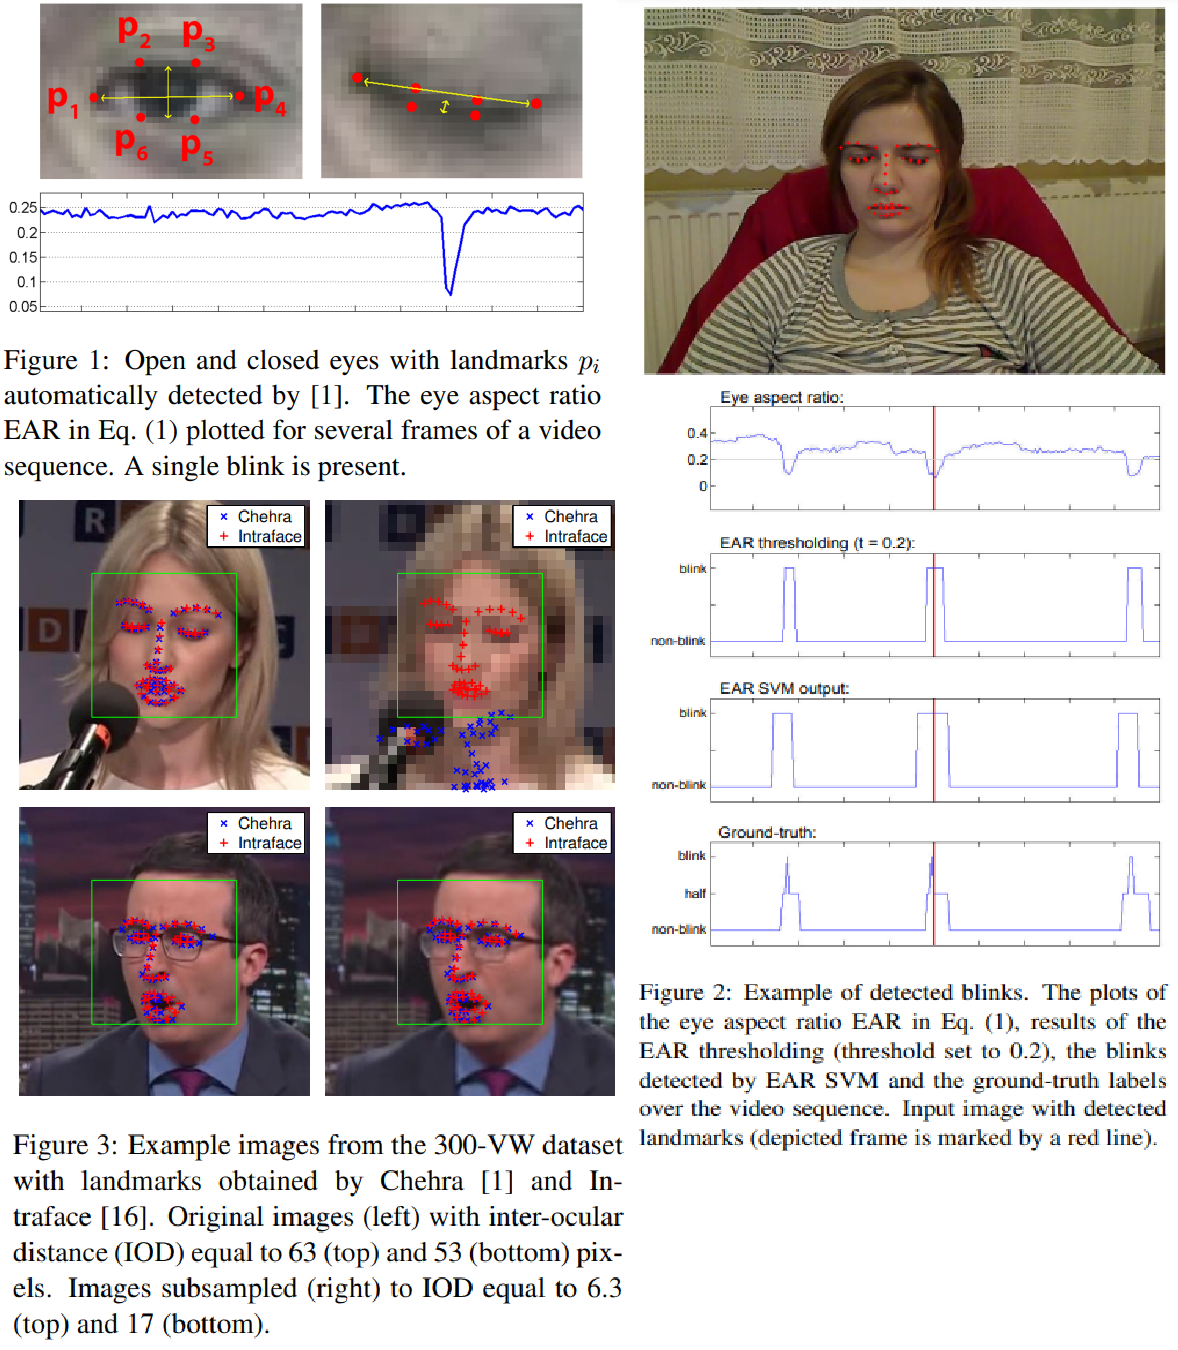
\includegraphics[width=0.80\textwidth]{img/ch3m1.png} 
\caption{实时检测标准摄像机视频序列中眨眼的算法}
\label{Test}
\end{figure}

Ching-Hua Weng 等人 \cite{weng2016driver} 提出了针对挑战赛特别会议使用 NTHU 计算机视觉实验室收集的驾驶员困倦视频数据集。整个包括训练、评估、测试的数据集包含 36 个不同种族的受试者在各种模拟驾驶场景下,所谓的场景包括正常驾驶、打哈欠、慢眨眼、入睡、爆笑记录等,而时间则在白天和夜间照明条件下都有。受试者坐在椅子上,用模拟的驱动轮和踏板玩简单的驾驶游戏时被记录下来;同时,他们在实验者的指导下进行一系列面部表情,整个数据集的总时间约为 9 个半小时。训练数据集包含 18 个主题,有 5 个 包含了 BareFace、Glasses、Night\_BareFace、Night\_Glasses、Sunglasses 的不同场景,也有每个受试者的序列,包括打哈欠和缓慢的眨眼频率,每个都记录大约 1 分钟。最后来对应于两个最重要场景的序列,嗜睡相关症状的组合如打哈欠、点头、缓慢眨眼和非嗜睡相关动作的组合如说话、大笑、看着两边,每个状态记录大约 1.5 分钟长,并评估和测试数据集包含 90 个驾驶视频(来自其他 18 名受试者),在不同场景下混合了困倦和非困倦状态。


\begin{figure}[htb]
\centering 
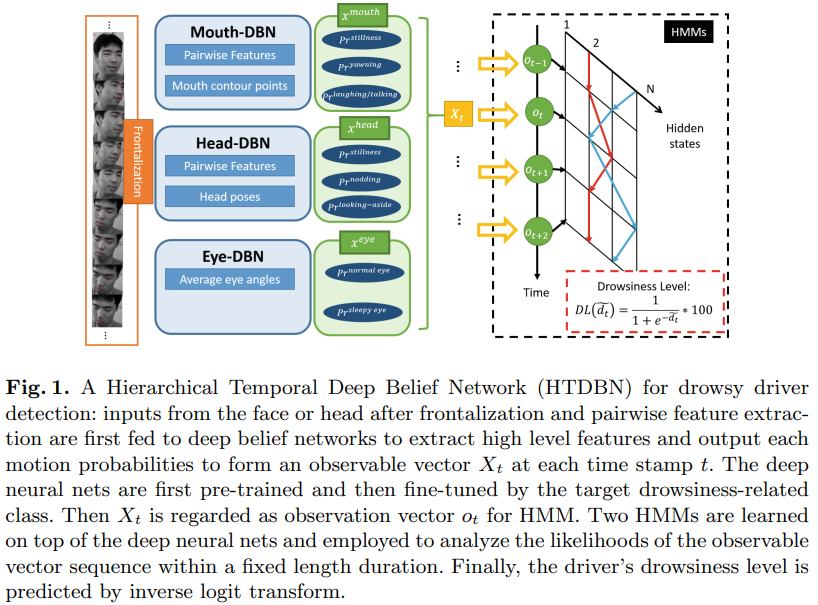
\includegraphics[width=0.80\textwidth]{img/ch3m2.png} 
\caption{A Hierarchical Temporal Deep Belief Network (HTDBN)}
\label{Test}
\end{figure}



X Luo 等人 \cite{luo2013driver} 采用不同的算法,即 AdaBoost 算法和红外帧差算法,在不同的行车光环境下定位眼睛的精确位置,研究者通过提取眼睛的特征参数来识别眼睛的状态,并基于 PERCLOS 的方法检测疲劳。同时,为了进一步测试驾驶员的疲劳程度,该研究使用局部二进制模式 (LBP) 算法来检测打哈欠作为辅助检测,其实验结果表明,该算法保证了系统的准确性,能够达到非接触式、不同光照条件和实时检测的要求。

Kaipeng Zhang 等人 \cite{zhang2016joint} 考量到由于各种姿势、照明和遮挡,在不受约束的环境中进行人脸检测和对齐上具有挑战性,而在最近的研究表明,深度学习方法可以在这两个任务上取得令人印象深刻的性能。该研究提出了一个深度级联多任务框架,利用框架它们之间的内在相关性来提高它们的性能。此外该研究框架采用级联结构,具有三个精心设计的深度卷积网络,以粗到细的方式预测人脸和地标位置。而在学习过程中,研究者提出了一种新的在线硬样本挖掘策略,可以自动提高性能,而无需手动选择样本。当中方法在具有挑战性的 FDDB 和 WIDER FACE 人脸检测基准以及用于人脸对齐的 AFLW 基准上实现了优于最先进技术的精度,同时保持了实时性能。